\begin{figure}[H]
    \captionsetup[subfigure]{justification=centering}
    \centering
    \begin{subfigure}[b]{0.45\textwidth}
        \centering
        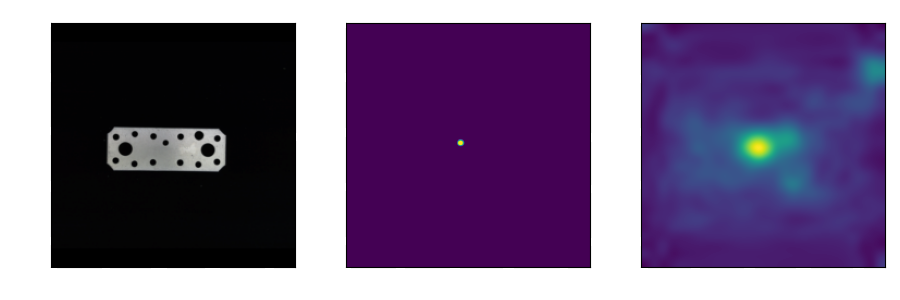
\includegraphics[width=\textwidth]{figures/overshootexamples/flat_connector_test_logical_anomalies_004.png}
        \caption{Example of overshooting image prediction.}

    \end{subfigure}
    \begin{subfigure}[b]{0.45\textwidth}
        \centering
        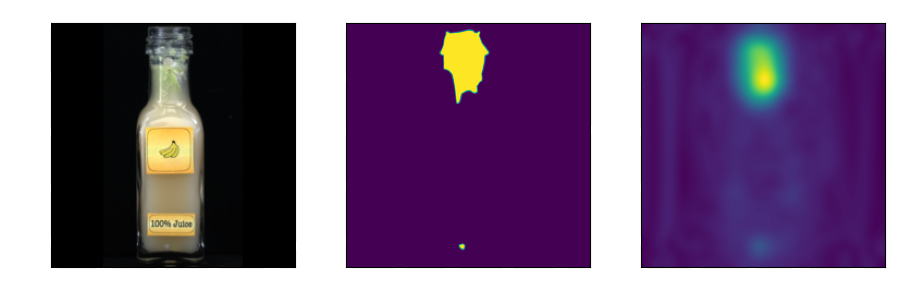
\includegraphics[width=\textwidth]{figures/overshootexamples/juice_bottle_test_structural_anomalies_019.png}
        \caption{Example of smaller anomalous region having significantly less certainty than larger regions.}

    \end{subfigure}
    
    \caption{Exemplary segmentations of representation-based classifiers that showcase less precise segmentaions than reconstruction-based approaches like DRAEM \cite{Zavrtanik_2021DRAEM}.}
    \label{fig:overshoot}
\end{figure}